\section{Results}
Many nice figures
\begin{enumerate}
	\item Histograms
	\item Histograms 3 directions
	\item PC
\end{enumerate}

\subsection{Activation Distribution on a  Fixed Force Vector}

\begin{figure}[ht]
   \begin{center}
    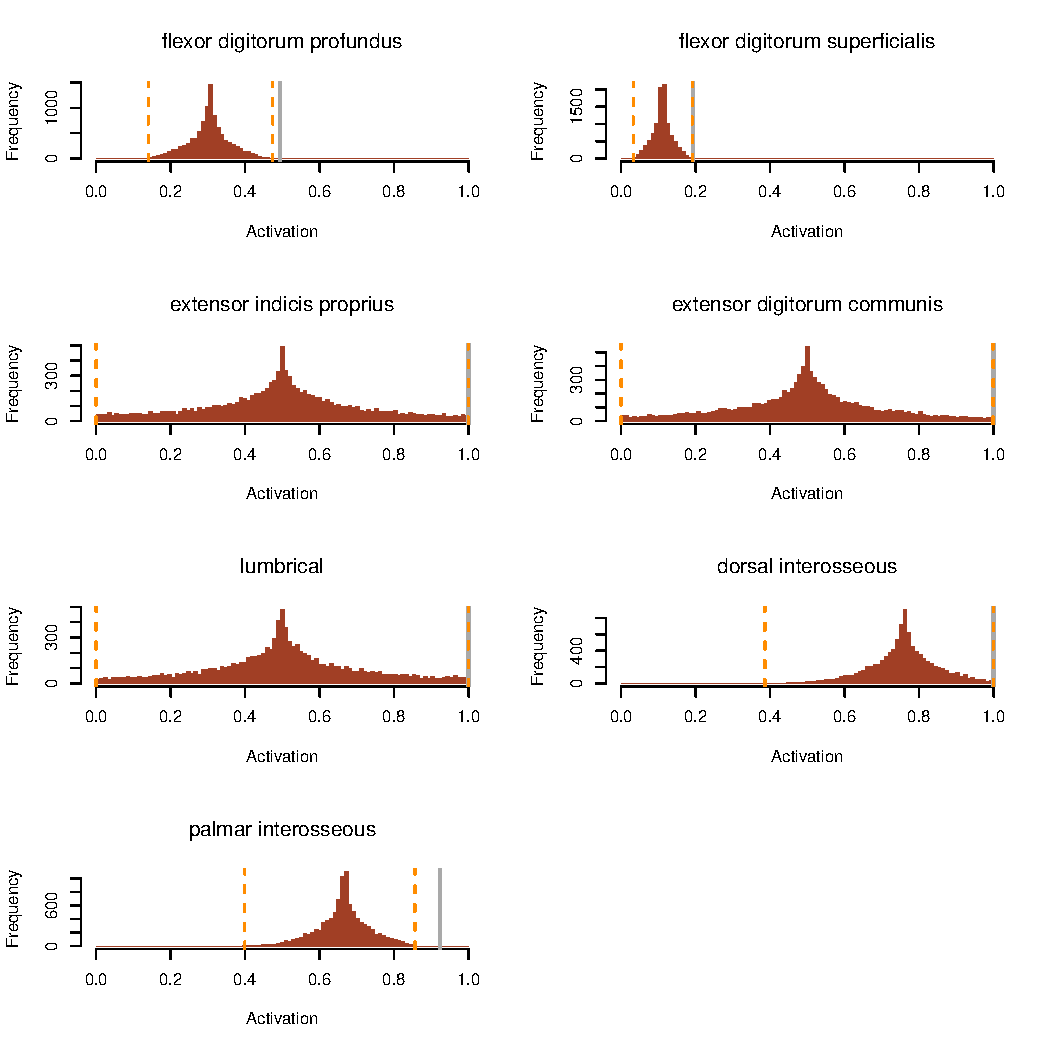
\includegraphics[width=0.5\textwidth]{figs/raw_histograms.pdf}
  \end{center}
  \caption{Histogram for Fixed Force}
  \label{fig_rawhisto}
\end{figure}

\subsection{Changing Output Force in 3 Directions}
We discuss different forces into three different directions, which are given by the palmar direction ($x$-direction), the distal direction ($y$-direction) and the sum of them. The maximal forces into each direction are given by ??, ?? and ?? respectively. For $\alpha = 0.1, 0.2, \dots, 0.9$, we give the histograms where the force is $\alpha \cdot F_{\max}$, where $F_{\max}$ is the maxium output force in the corresponding direction. 

\begin{figure}[!H]
   \begin{center}
    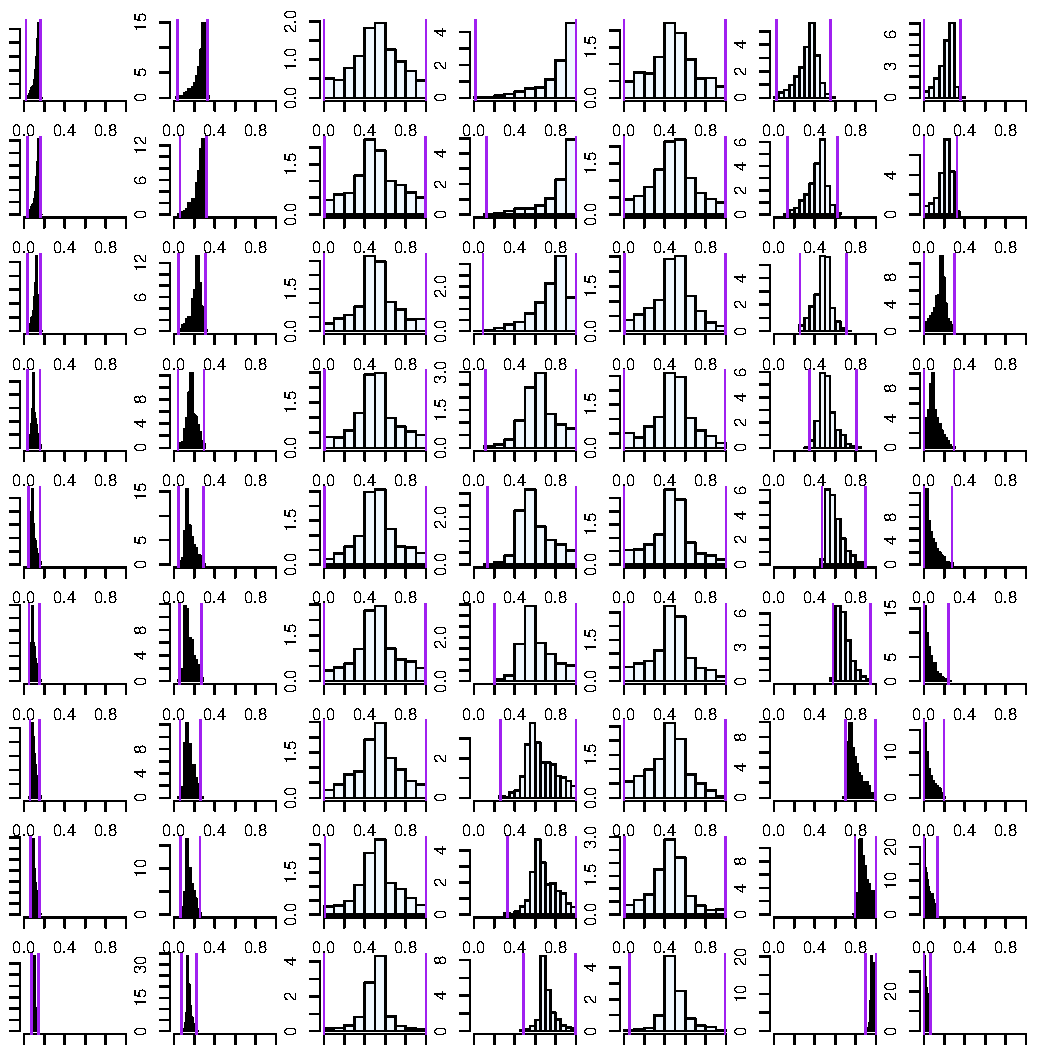
\includegraphics[width=1.0\textwidth]{figs/X_alphaProgression.pdf}
  \end{center}
  \caption{Histogram for $x$-Direction}
  \label{fig_xhisto}
\end{figure}

\begin{figure}[!H]
   \begin{center}
    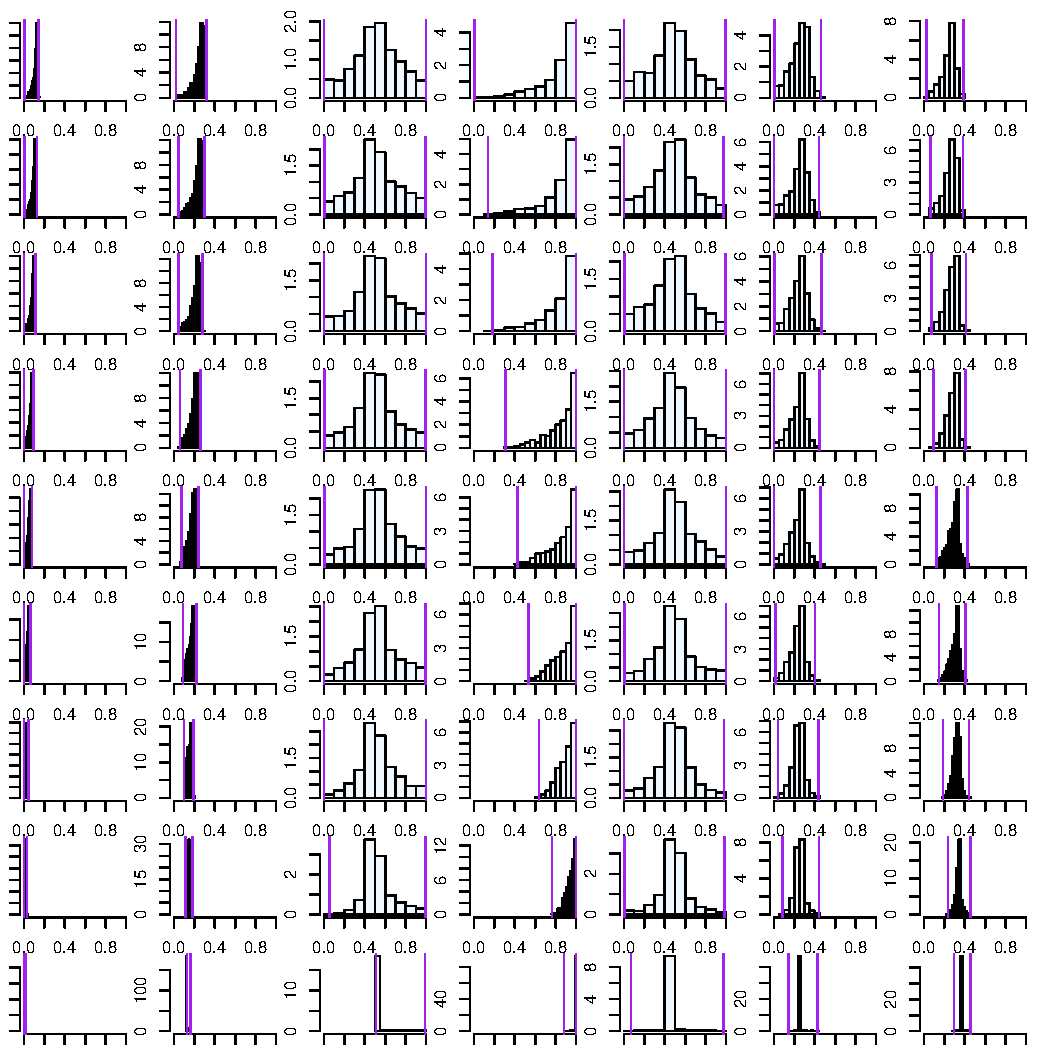
\includegraphics[width=1.0\textwidth]{figs/Y_alphaProgression.pdf}
  \end{center}
  \caption{Histogram for $xy$-Direction}
  \label{fig_yhisto}
\end{figure}

\begin{figure}[!H]
   \begin{center}
    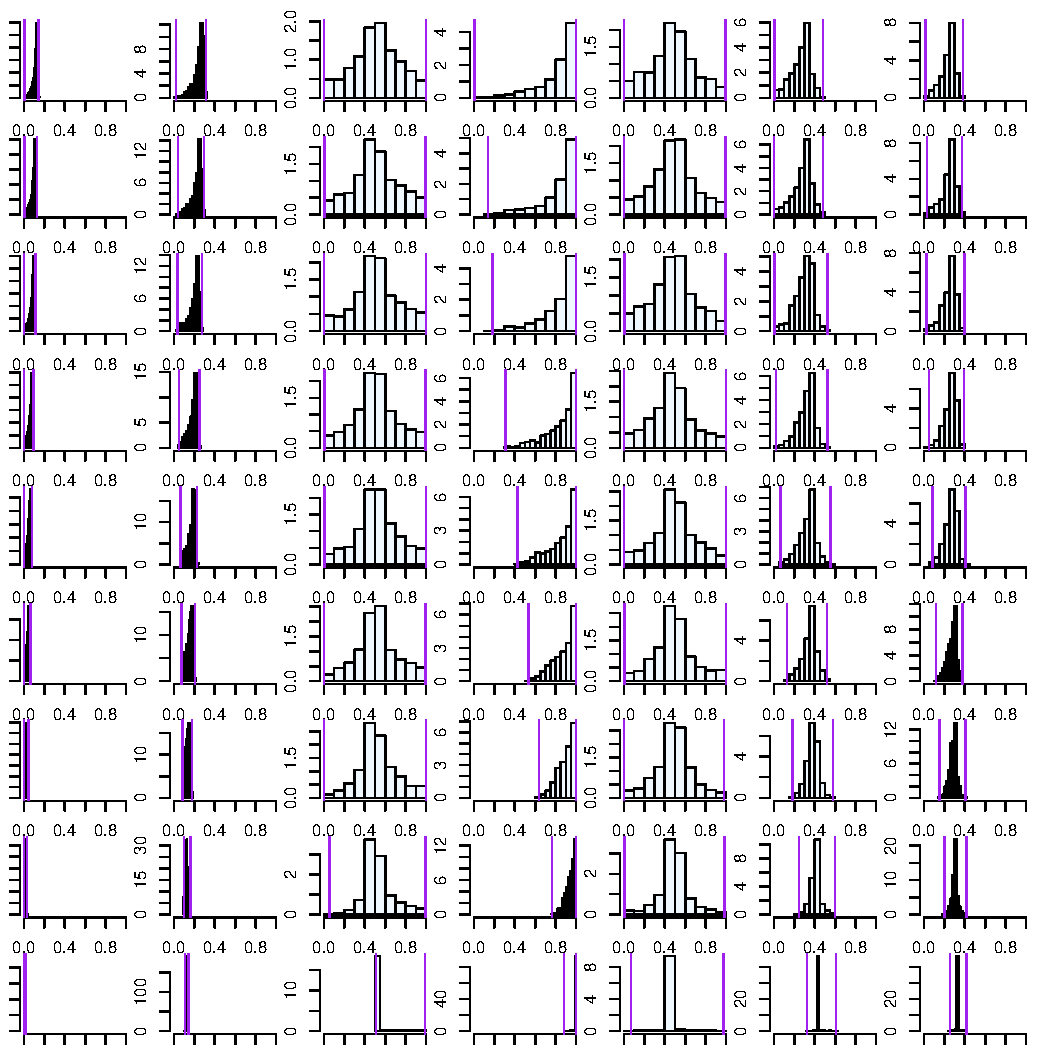
\includegraphics[width=1.0\textwidth]{figs/XY_alphaProgression.pdf}
  \end{center}
  \caption{Histogram for $xy$-Direction}
  \label{fig_xyhisto}
\end{figure}

\subsection{Parallel Coordinates}

\begin{figure}[ht]
   \begin{center}
    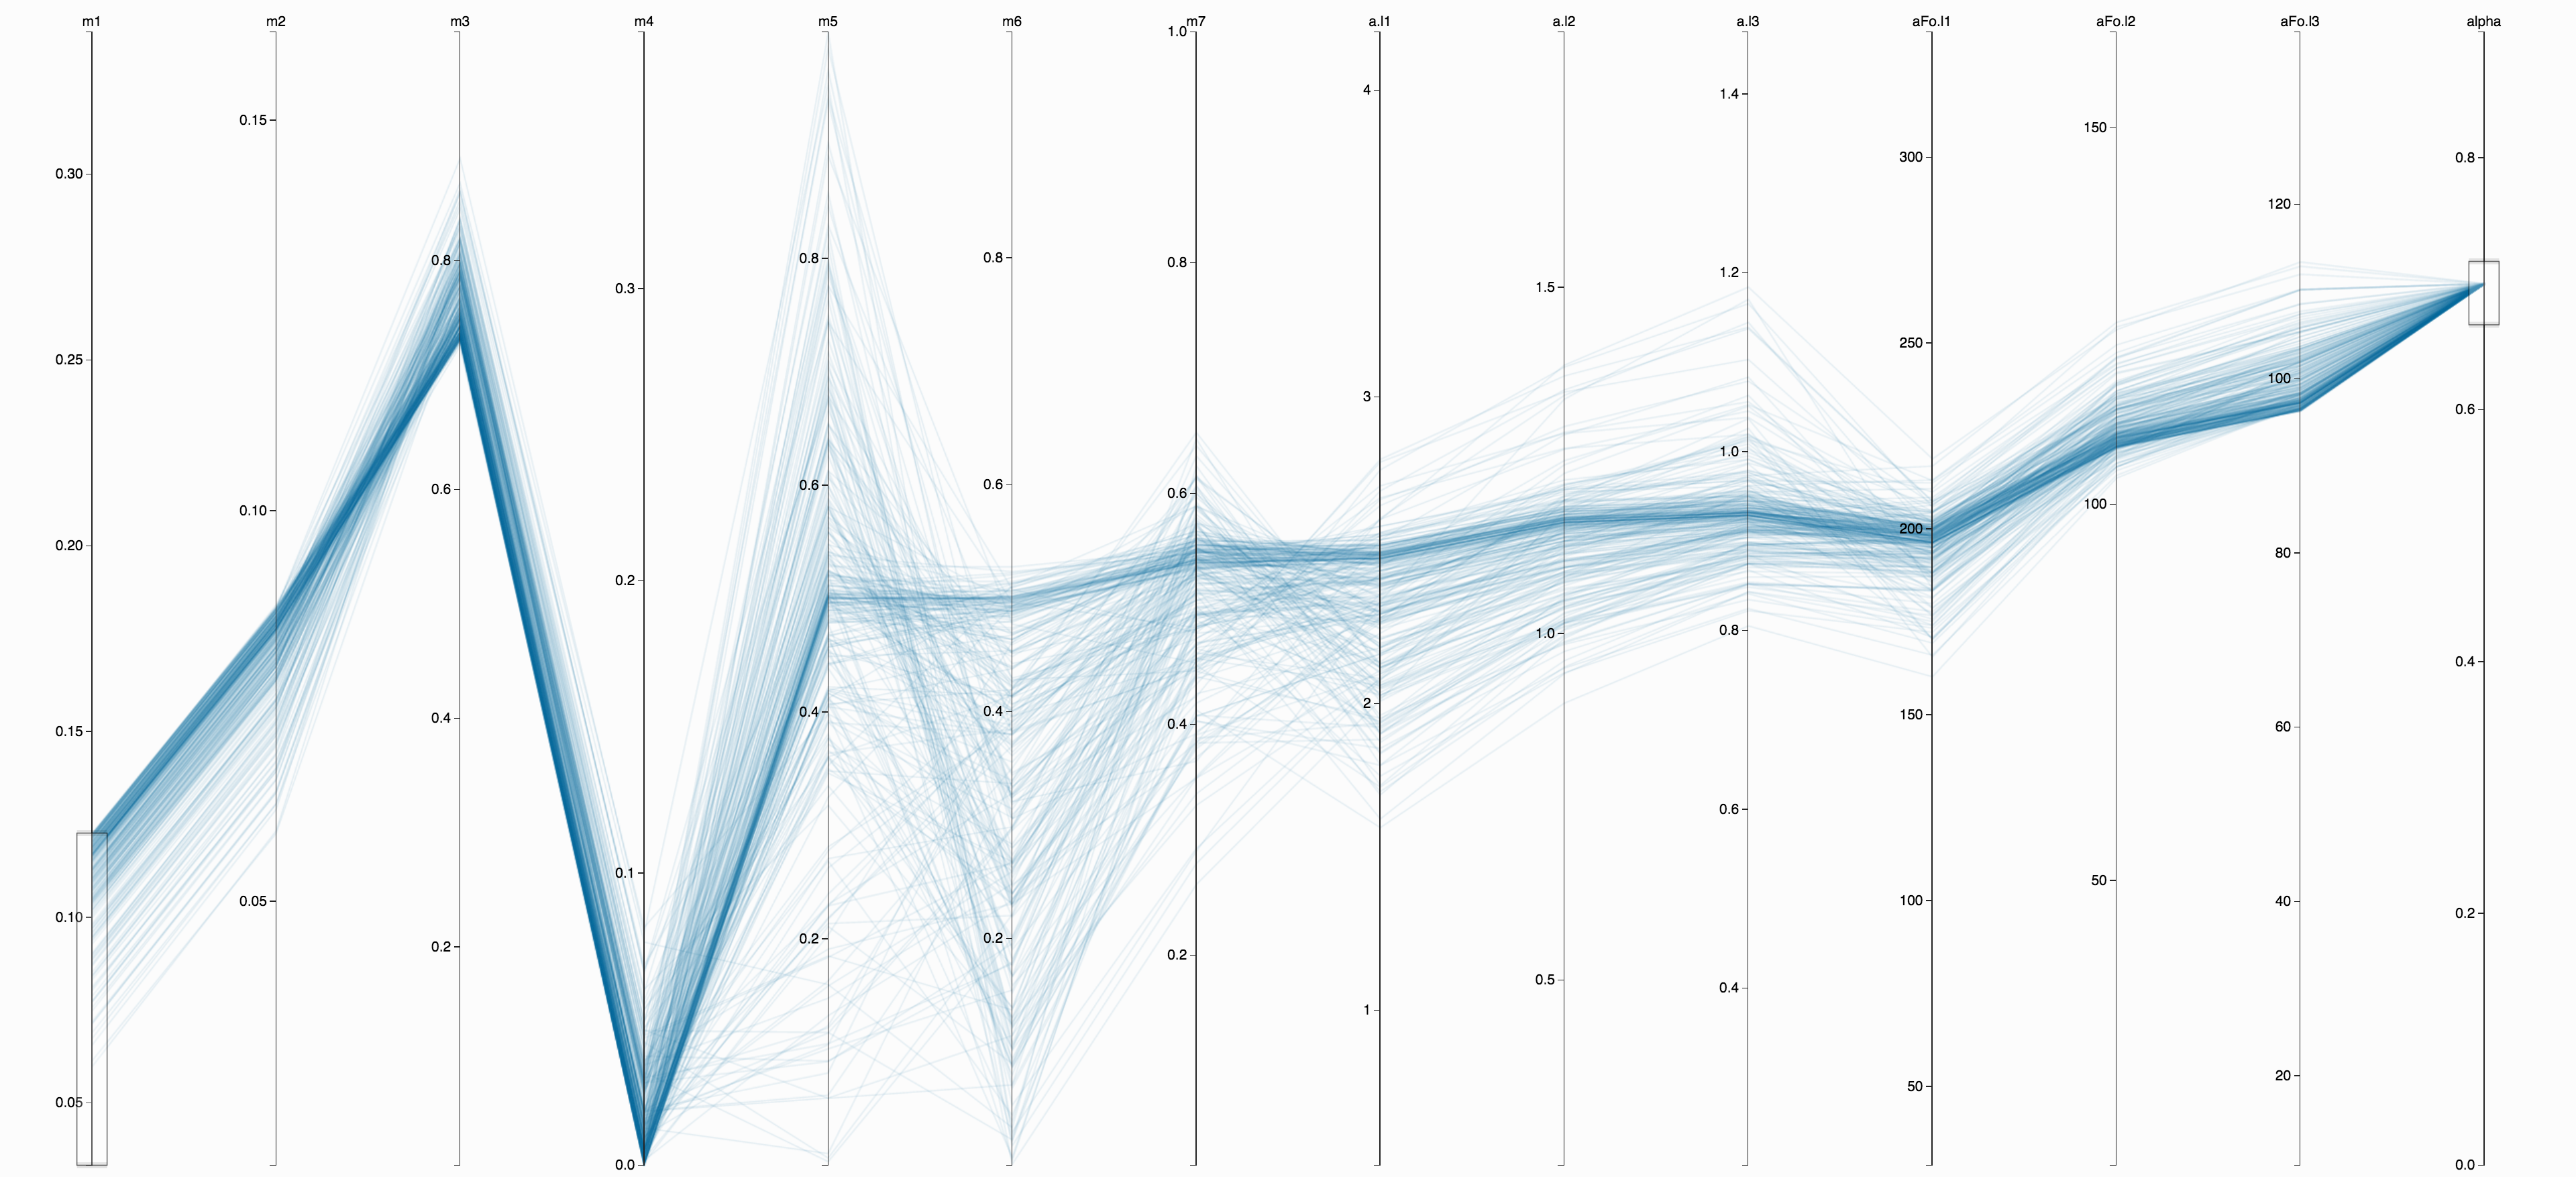
\includegraphics[width=1.0\textwidth]{figs/X_a8_lower.png}
  \end{center}
  \caption{Low for Muscle 1}
  \label{fig_low}
\end{figure}

\begin{figure}[ht]
   \begin{center}
    \includegraphics[width=1.0\textwidth]{figs/X_a8_middle.png}
  \end{center}
  \caption{Middle for Muscle 1}
  \label{fig_mid}
\end{figure}

\begin{figure}[ht]
   \begin{center}
    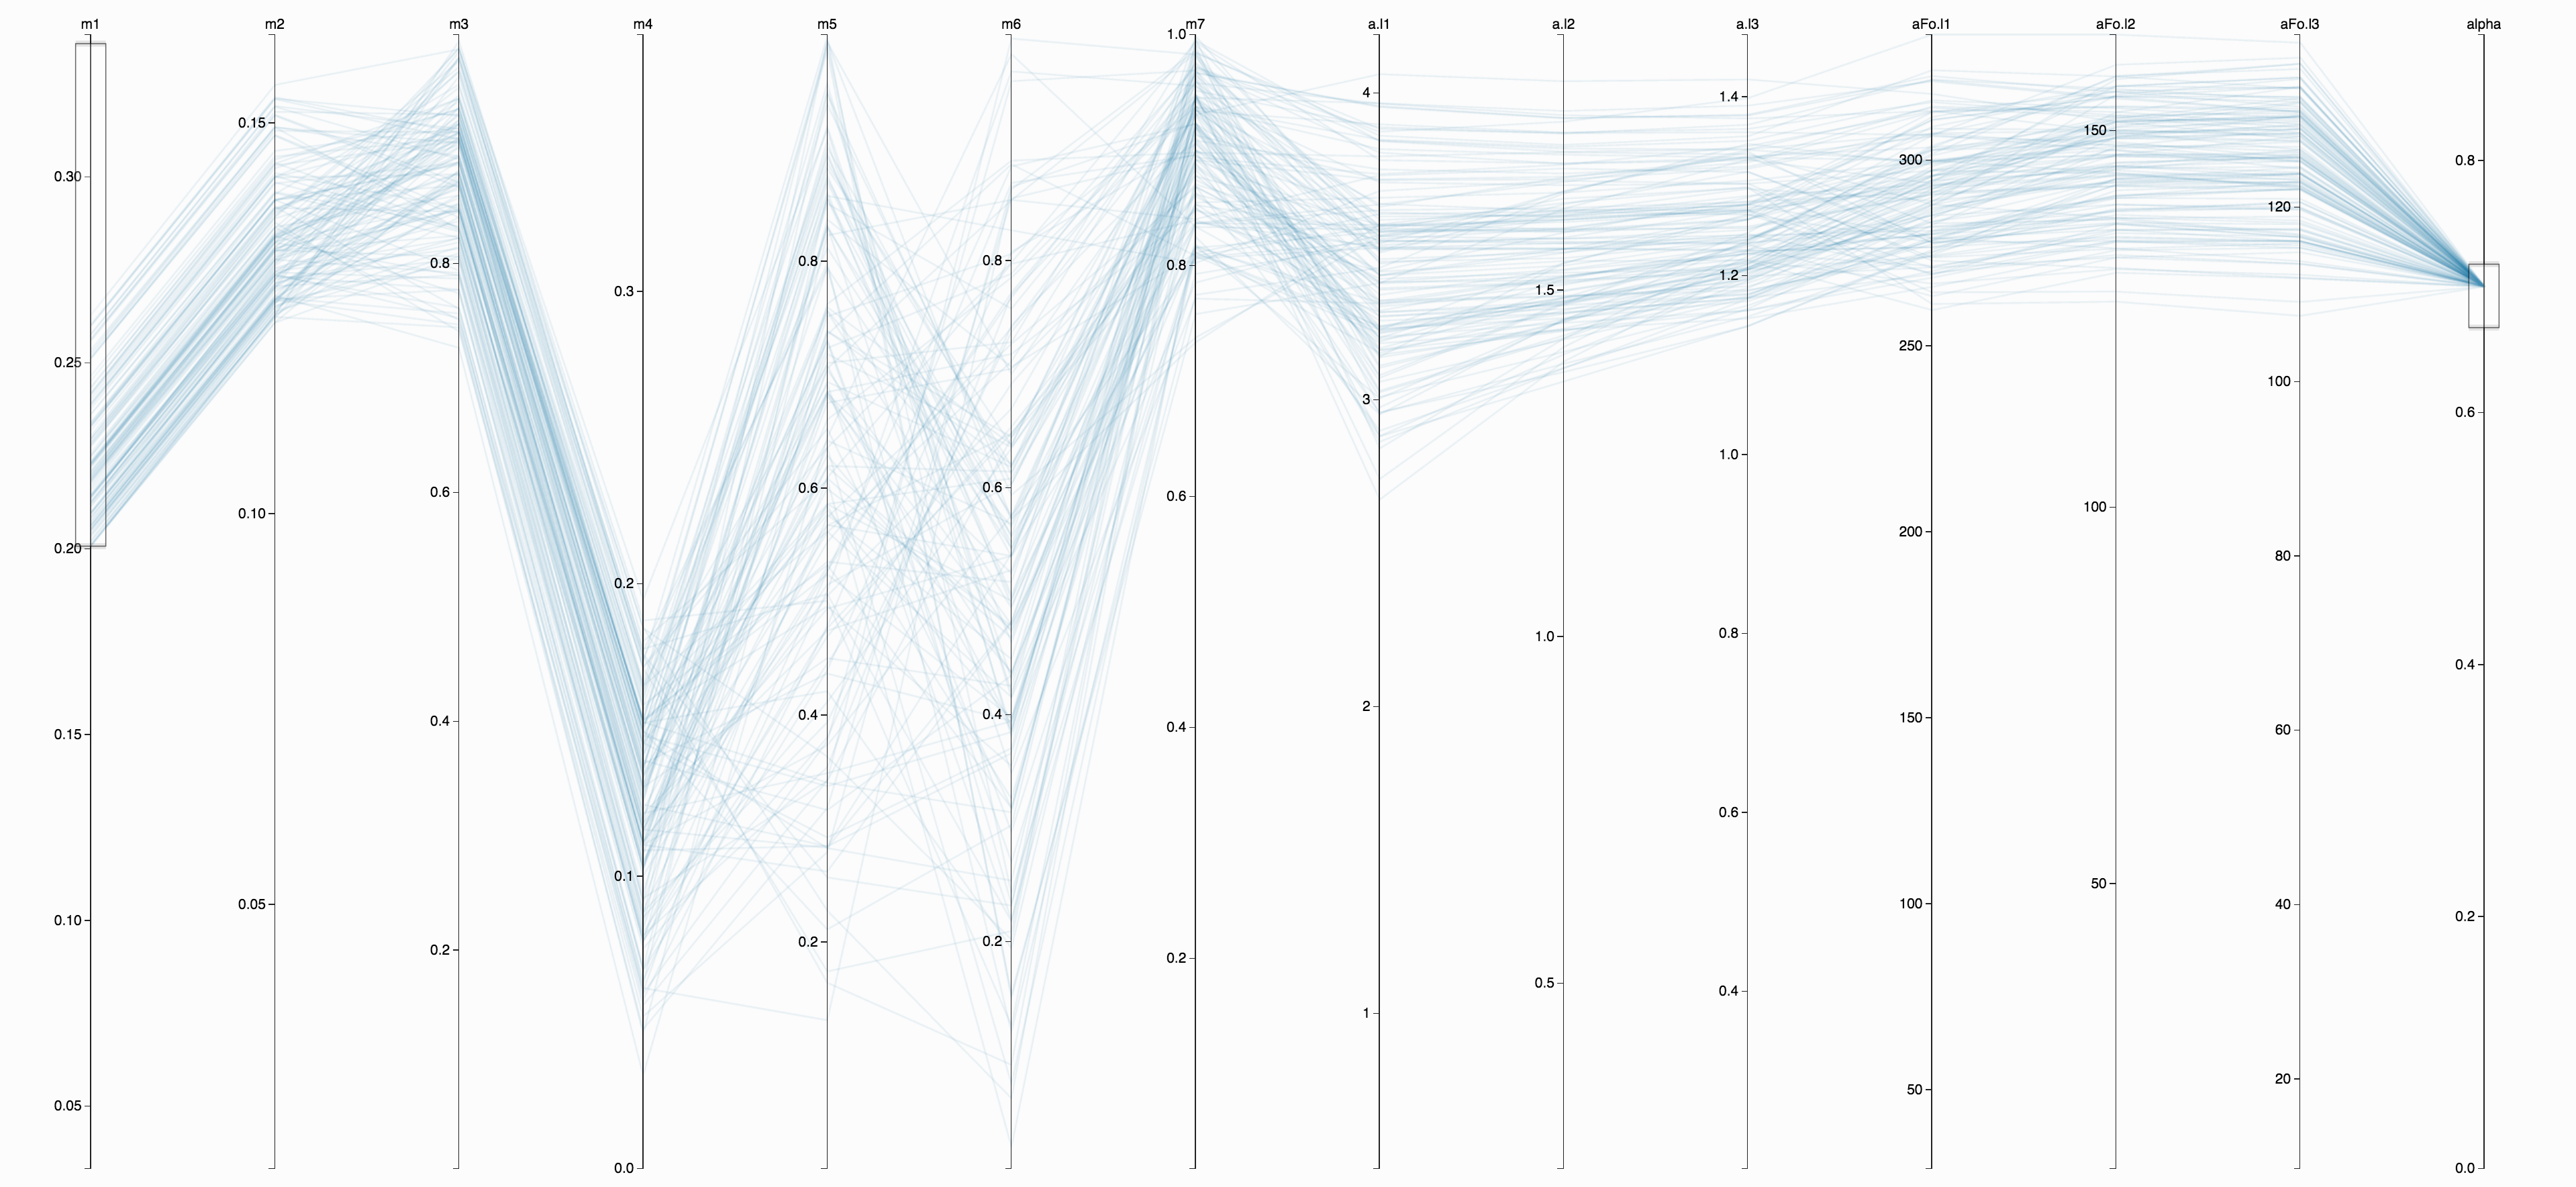
\includegraphics[width=1.0\textwidth]{figs/X_a8_upper.png}
  \end{center}
  \caption{Upper for Muscle 1}
  \label{fig_high}
\end{figure}

\begin{figure}[ht]
   \begin{center}
    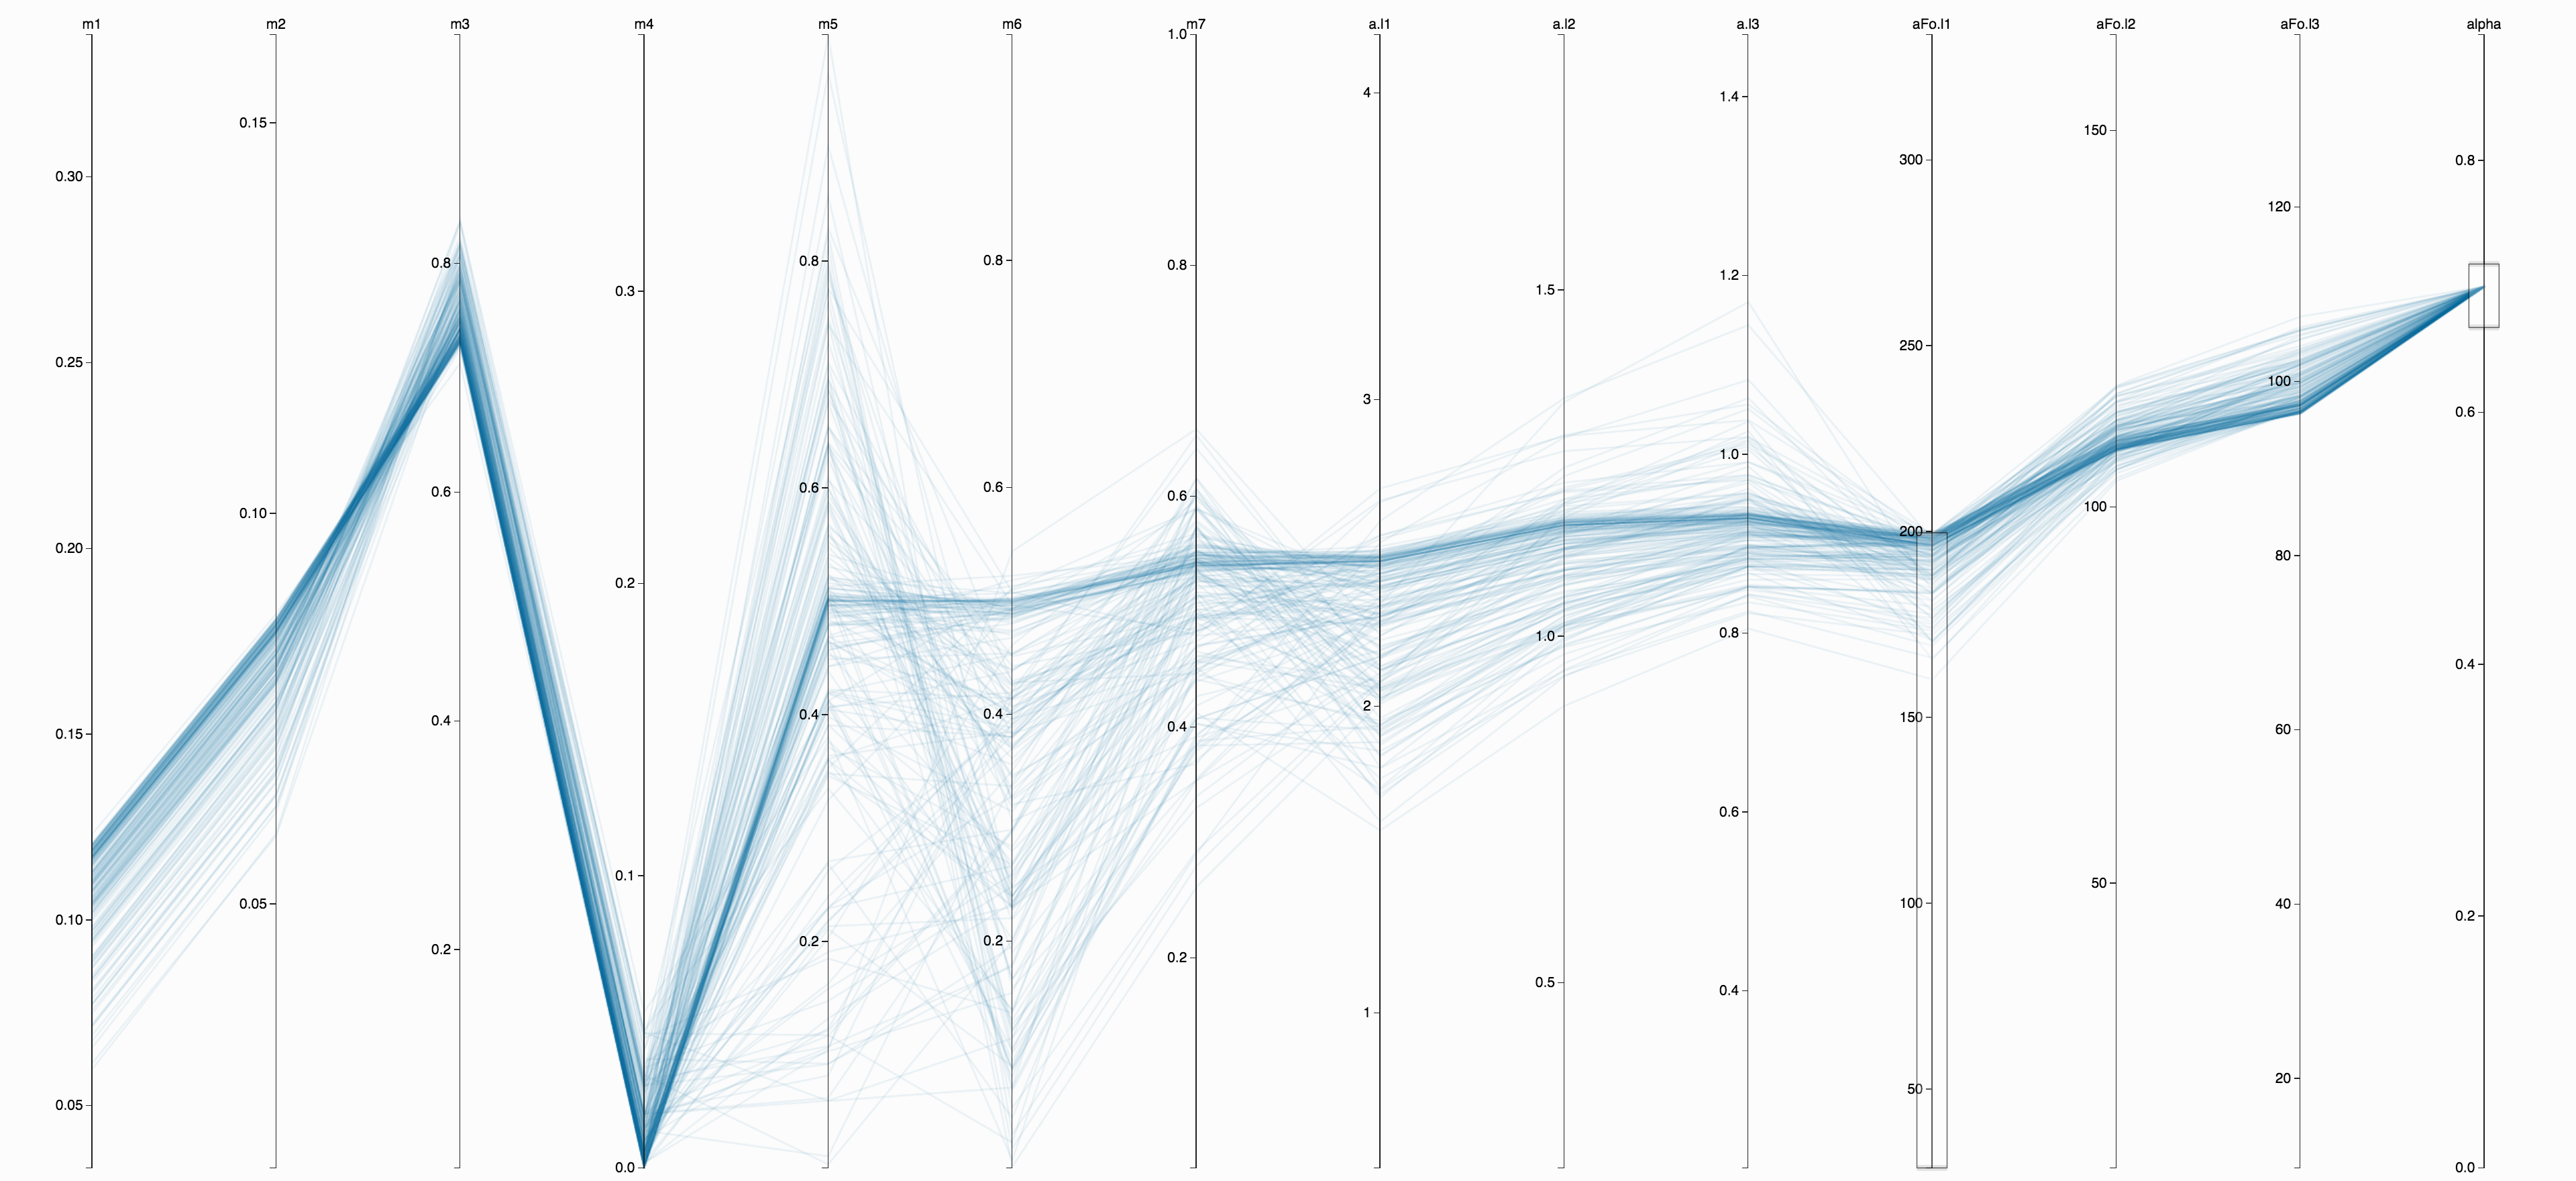
\includegraphics[width=1.0\textwidth]{figs/X_a8_weightedcost.png}
  \end{center}
  \caption{Weighted Cost}
  \label{fig_cost}
\end{figure}

\textit{Muscle 5 and 6 same direction and same strength $\Rightarrow$ Does not matter which one we activate for low cost}